\documentclass{standalone}
\usepackage{pgfplots}


\begin{document}

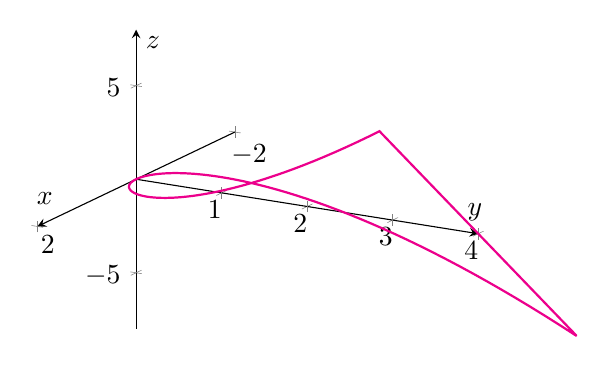
\begin{tikzpicture}
    \begin{axis}[
        xlabel={$x$},
        ylabel={$y$},
        zlabel={$z$},
        axis lines=center,
        view={120}{20}, % Adjust the view angle as needed
        domain=-2:2,    % Adjust the range of 't' as needed
        samples=100,    % Number of points to sample
        unbounded coords=jump, % Prevent connecting the first and last points
        ]
        \addplot3[
            magenta,    % Change the color to magenta
            thick,      % Make the line thick
            variable=t,
            parametric,
        ] ({t}, {t^2}, {t^3});
    \end{axis}
\end{tikzpicture}

\end{document}
